\index{MMS} \index{method of manufactured solutions}

The method of manufactured solutions is a relatively simple way of carrying out
code verification. In essence, one postulates a solution for the PDE at hand (as
well as the proper boundary conditions), inserts it in the PDE and computes the 
corresponding source term. 
The same source term and boundary conditions will then be used in a numerical 
simulation so that the computed solution can be compared with the (postulated)
true analytical solution. 

Examples of this approach are to be found in \cite{dohu,busa13,bodg06}.


%-----------------------------------------------------------------------------
\subsubsection{Analytical benchmark I \label{mms1}}

Taken from \cite{dohu03}. We consider a two-dimensional problem 
in the square domain $\Omega=[0,1]\times[0,1]$, which possesses a closed-form analytical 
solution. The problem consists of determining the velocity field ${\vec \upnu} = (u,v)$ 
and the pressure $p$ such that 
\begin{eqnarray}
\eta \Delta {\vec \upnu} - {\vec \nabla} p + {\vec b} &=& \vec 0 \quad\quad {\rm in} \; \Omega\\
\vec{\nabla} \cdot \vec{v} &=& 0 \quad\quad {\rm in} \; \Omega\\
\vec{v}&=&\vec{0} \quad\quad {\rm on} \; \Gamma_D
\end{eqnarray}
where the fluid viscosity is taken as $\eta=1$.
The components of the body force $\vec{b}$ are prescribed as 
\begin{eqnarray}
b_x &=& (12 - 24y) x^4 + (-24 + 48y) x^3 + (-48y + 72y^2 - 48 y^3 + 12) x^2 \nonumber\\
    && + (-2 + 24y -72y^2+48y^3)x + 1-4y + 12y^2-8y^3 \nonumber\\ 
b_y &=& (8 - 48y + 48 y^2) x^3 + (-12 + 72y - 72y^2) x^2  \nonumber\\
    && + (4 - 24y + 48y^2 - 48y^3 + 24y^4) x - 12y^2 + 24y^3 - 12y^4  \nonumber
\end{eqnarray}
With this prescribed body force, the exact solution is 
\begin{eqnarray}
u(x,y) &=& x^2(1- x)^2 (2y - 6y^2 + 4y^3)  \nonumber\\
v(x,y) &=& -y^2 (1 - y)^2 (2x - 6x^2 + 4x^3) \nonumber\\
p(x,y) &=& x(1 -x)- 1/6 \nonumber 
\end{eqnarray}
Note that the pressure obeys $\int_{\Omega} p \; d\Omega = 0$.
One can turn to the spatial derivatives of the fields:
\begin{eqnarray}
\frac{\partial u}{\partial x} &=&  (2x -6x^2 +4 x^3 ) (2y - 6y^2 + 4y^3)  \\
\frac{\partial v}{\partial y} &=&  - (2x -6x^2 +4 x^3 ) (2y - 6y^2 + 4y^3)  
\end{eqnarray}
with of course  ${\vec \nabla} \cdot {\vec \upnu} = 0$ and 
\begin{eqnarray}
\frac{\partial p}{\partial x} &=& 1-2x  \\
\frac{\partial p}{\partial y} &=& 0
\end{eqnarray}

The velocity and pressure fields look like:

\begin{center}
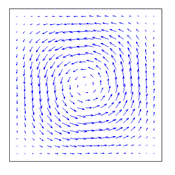
\includegraphics[height=4cm]{images/mms/Ex1_Q2Q1_velo.png}
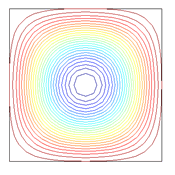
\includegraphics[height=4cm]{images/mms/Ex1_Q2Q1_streamlines.png}
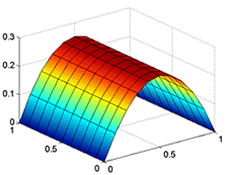
\includegraphics[height=4cm]{images/mms/Ex1_Q2Q1_pres.png}\\
{\small http://ww2.lacan.upc.edu/huerta/exercises/Incompressible/Incompressible\_Ex1.htm}
\end{center}

As shown in \cite{dohu03}, If the LBB condition is not satisfied, spurious oscillations spoil the pressure approximation. 
Figures below show results obtained with a mesh of 20x20 Q1P0 (left) and P1P1 (right) elements:
\begin{center}
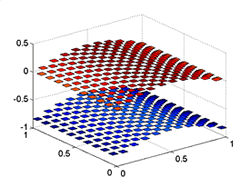
\includegraphics[height=5cm]{images/mms/Ex1_Q1P0_pres.png}
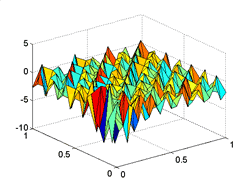
\includegraphics[height=5cm]{images/mms/Ex1_P1P1_pres.png}]]
{\small http://ww2.lacan.upc.edu/huerta/exercises/Incompressible/Incompressible\_Ex1.htm}
\end{center}

Taking into account that the proposed problem has got analytical solution, it is easy to analyze convergence of the different pairs of elements:
\begin{center}
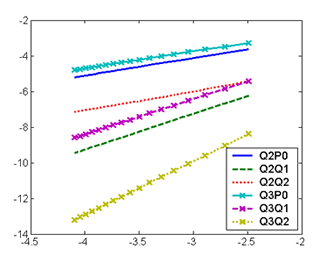
\includegraphics[height=7cm]{images/mms/Ex1_conv_qua.png}\\
{\small http://ww2.lacan.upc.edu/huerta/exercises/Incompressible/Incompressible\_Ex1.htm}
\end{center}




%-----------------------------------------------------------------------------
\subsubsection{Analytical benchmark II \label{mms2}}

Taken from \cite{dobo04}. It is for a unit square with $\nu=\mu/\rho=1$ and the smooth exact solution is
\begin{eqnarray}
u(x,y) &=& x+x^2 - 2xy+x^3 - 3xy^2 + x^2y \\
v(x,y) &=& -y-2xy+y^2 -3x^2y + y^3 - xy^2 \\
p(x,y) &=& xy+x+y+x^3y^2 - 4/3
\end{eqnarray}
Note that the pressure obeys $\int_{\Omega} p \; d\Omega = 0$

\begin{eqnarray}
b_x &=& - (1+y-3x^2y^2) \\
b_y &=& - (1-3x-2x^3y) 
\end{eqnarray}


%-----------------------------------------------------------------------------
\subsubsection{Analytical benchmark III \label{mms3}}

This benchmark begins by postulating a polynomial solution 
to the 3D Stokes equation \cite{dobo04}:
\begin{equation}
{\bm v}
=
\left(
\begin{array}{c}
x+x^2+xy+x^3y \\
y + xy + y^2 + x^2 y^2\\
-2z - 3xz - 3yz - 5x^2 yz
\end{array}
\right)
\label{eqbur}
\end{equation}
and
\begin{equation}
p = xyz + x^3 y^3z - 5/32
\end{equation}
While it is then trivial to verify that this velocity field is divergence-free,  
the corresponding body force of the Stokes equation can be computed by  
inserting this solution into the momentum equation with a given viscosity $\mu$
(constant or position/velocity/strain rate dependent). 
The domain is a unit cube and velocity boundary conditions 
simply use Eq. (\ref{eqbur}). 
Note that the pressure fulfills 
\[
\int_\Omega p({\vec r}) d\Omega = 0.  
\]


\paragraph{Constant viscosity}
In this case, the right hand side writes:
\begin{eqnarray}
{\bm f} &=& 
-{\bm \nabla p} + 
\mu
\left(
\begin{array}{c}
2+6xy \\
2+2x^2+2y^2 \\
-10yz
\end{array}
\right) \nonumber\\
&=&
-
\left(
\begin{array}{c}
yz+3x^2 y^3z \\
xz+3 x^3 y^2 z \\
xy+x^3y^3
\end{array}
\right) 
+
\mu
\left(
\begin{array}{c}
2+6xy \\
2+2x^2+2y^2 \\
-10yz
\end{array}
\right)
\nonumber
\end{eqnarray}

We can compute the components of the strainrate tensor:
\begin{eqnarray}
\dot{\varepsilon}_{xx} &=& 1+2x+y+3x^2y\\
\dot{\varepsilon}_{yy} &=& 1+x+2y+2x^2y\\
\dot{\varepsilon}_{zz} &=& -2-3x-3y-5x^2y\\ 
\dot{\varepsilon}_{xy} &=&  \frac{1}{2} (x+y+2xy^2+x^3)\\
\dot{\varepsilon}_{xz} &=&  \frac{1}{2} (-3z-10xyz  )\\
\dot{\varepsilon}_{yz} &=&  \frac{1}{2} ( -3z -5x^2z )
\end{eqnarray}
Note that we of course have $\dot{\varepsilon}_{xx} +\dot{\varepsilon}_{yy} 
+\dot{\varepsilon}_{zz} =0$.

\paragraph{Variable viscosity}

In this case, the right hand side is obtains through
\begin{eqnarray}
{\bm f} &=& -{\bm \nabla p} + 
\mu
\left(
\begin{array}{c}
2+6xy \\
2+2x^2+2y^2 \\
-10yz
\end{array}
\right) \nonumber\\
&+&
\left(
\begin{array}{c}
2 \dot{\varepsilon}_{xx} \\
2 \dot{\varepsilon}_{xy} \\
2 \dot{\varepsilon}_{xz}
\end{array}
\right) \frac{\partial \mu}{\partial x}
+
\left(
\begin{array}{c}
2 \dot{\varepsilon}_{xy} \\
2 \dot{\varepsilon}_{yy} \\
2 \dot{\varepsilon}_{yz}
\end{array}
\right) \frac{\partial \mu}{\partial y}
+
\left(
\begin{array}{c}
2 \dot{\varepsilon}_{xz} \\
2 \dot{\varepsilon}_{yz} \\
2 \dot{\varepsilon}_{zz} 
\end{array}
\right) \frac{\partial \mu}{\partial z}
\end{eqnarray}


The viscosity can be chosen to be a smooth varying function:
\begin{equation}
\mu = exp(1 - \beta(x(1 - x) + y(1 - y) + z(1 - z)))
\end{equation}
Choosing $\beta=0$ yields a constant velocity $\mu=e^1$ (and greatly simplifies the right-hand side).
One can easily show that the ratio of viscosities $\mu^\star$
in the system follows $\mu^\star=\exp(-3\beta/4)$ so that choosing $\beta=10$ yields
$\mu^\star\simeq 1808$ and $\beta=20$ yields $\mu^\star\simeq 3.269\times10^6$.
In this case
\begin{eqnarray}
\frac{\partial \mu}{\partial x}&=&-4\beta(1-2x)\mu(x,y,z)\\
\frac{\partial \mu}{\partial y}&=&-4\beta(1-2y)\mu(x,y,z)\\
\frac{\partial \mu}{\partial z}&=&-4\beta(1-2z)\mu(x,y,z)
\end{eqnarray}


\cite{busa13} has carried out this benchmark for $\beta=4$, i.e.: 
\[
\mu(x,y,z)=\exp ( 1-4( x(1-x)+y(1-y)+z(1-z)  )  )
\]
In a unit cube, this yields a variable viscosity such that
$0.1353 < \mu <   2.7182$, i.e. a ratio of approx. 20 within the domain. We then have:
\begin{eqnarray}
\frac{\partial \mu}{\partial x}&=&-4(1-2x)\mu(x,y,z)\\
\frac{\partial \mu}{\partial y}&=&-4(1-2y)\mu(x,y,z)\\
\frac{\partial \mu}{\partial z}&=&-4(1-2z)\mu(x,y,z)
\end{eqnarray}

\todo[inline]{sort out mess wrt Eq 26 of busa13}


%-----------------------------------------------------------------------------
\subsubsection{Analytical benchmark IV \label{mms4}}

From \cite{been79}. The two-dimensional domain is a unit square. The body forces are:
\begin{eqnarray}
f_x &=& 128[ x^2(x-1)^2 12 (2y-1) + 2 (y-1)(2y-1)y(12x^2-12x+2)  ] \nn\\
f_y &=& 128[ y^2(y-1)^2 12 (2x-1) + 2 (x-1)(2x-1)y(12y^2-12y+2)  ] \nn\\
\end{eqnarray}
The solution is
\begin{eqnarray}
u &=& -256x^2(x-1)^2y(y-1)(2y-1) \nn\\
v &=&  256x^2(y-1)^2x(x-1)(2x-1) \nn\\
p &=& 0 
%p &=& (x-1/2)(y-1/2) 
\end{eqnarray}

Another choice:
\begin{eqnarray}
f_x &=& 128[ x^2(x-1)^2 12 (2y-1) + 2 (y-1)(2y-1)y(12x^2-12x+2)  ] + y - 1/2 \nn\\
f_y &=& 128[ y^2(y-1)^2 12 (2x-1) + 2 (x-1)(2x-1)y(12y^2-12y+2)  ] + x - 1/2 \nn\\
\end{eqnarray}
The solution is
\begin{eqnarray}
u &=& -256x^2(x-1)^2y(y-1)(2y-1) \nn\\
v &=&  256x^2(y-1)^2x(x-1)(2x-1) \nn\\
p &=& (x-1/2)(y-1/2) 
\end{eqnarray}


%-----------------------------------------------------------------------------
\subsubsection{Analytical benchmark V \label{mms5}}

This is taken from Appendix D1 of \cite{john16}.

The domain $\Omega$ is a unit square. We consider the stream function
\[
\phi(x,y)=1000x^2(1-x)^4y^3(1-y)^2
\]
The velocity field is defined by
\begin{eqnarray}
u(x,y) &=&  \partial_y \phi = 1000(x^2(1-x)^4 y^2 (1-y)(3-5y)  ) \\
v(x,y) &=& -\partial_x \phi = 1000(-2x(1-x)^3(1-3x)y^3(1-y)^2)
\end{eqnarray}
and it is easy to verify that $\vec\nabla\cdot\vec v=0$.

The pressure is given by:
\[
p(x,y)=\pi^2( xy^3\cos(2\pi x^2y) - x^2y \sin(2\pi xy)) + \frac{1}{8}
\]

\begin{center}
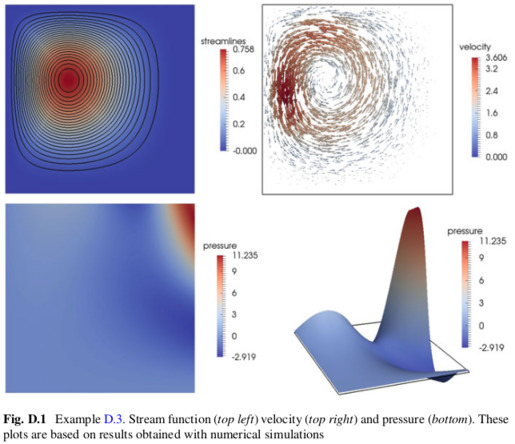
\includegraphics[width=8cm]{images/mms/mms5}\\
Taken from \cite{john16}.
\end{center}



